\documentclass[12pt,openany,a4paper]{book}
\usepackage{graphics} % for pdf, bitmapped graphics files
\usepackage{epsfig} % for postscript graphics files
\usepackage{mathptmx} % assumes new font selection scheme installed
\usepackage{times} % assumes new font selection scheme installed
\usepackage{amsmath} % assumes amsmath package installed
\usepackage{amssymb}  % assumes amsmath package installed
\usepackage[export]{adjustbox}
\usepackage{stfloats}% if you want encapsulated PS figures.

% If you use a macro file called macros.tex :
% \input{macros}
% Note: The present document has its macros built in.

% Number subsections but not subsubsections:
\setcounter{secnumdepth}{2}
% Show subsections but not subsubsections in table of contents:
\setcounter{tocdepth}{2}

\pagestyle{headings}		% Chapter on left page, Section on right.
\raggedbottom

\setlength{\topmargin}		{-5mm}  %  25-5 = 20mm
\setlength{\oddsidemargin}	{10mm}  % rhs page inner margin = 25+10mm
\setlength{\evensidemargin}	{0mm}   % lhs page outer margin = 25mm
\setlength{\textwidth}		{150mm} % 35 + 150 + 25 = 210mm
\setlength{\textheight}		{240mm} % 

\renewcommand{\baselinestretch}{1.2}	% Looks like 1.5 spacing.

% Stop figure/tables smaller than 3/4 page from appearing alone on a page:
\renewcommand{\textfraction}{0.25}
\renewcommand{\topfraction}{0.75}
\renewcommand{\bottomfraction}{0.75}
\renewcommand{\floatpagefraction}{0.75}

% THEOREM-LIKE ENVIRONMENTS:
\newtheorem{defn}	{Definition}	% cf. \dfn for cross-referencing
\newtheorem{theorem}	{Theorem}	% cf. \thrm for cross-referencing
\newtheorem{lemma}	{Lemma}		% cf. \lem for cross-referencing

% AIDS TO CROSS-REFERENCING (All take a label as argument):
\newcommand{\eref}[1] {(\ref{#1})}		% (...)
\newcommand{\eq}[1]   {Eq.\,(\ref{#1})}		% Eq.~(...)
\newcommand{\eqs}[2]  {Eqs.~(\ref{#1}) and~(\ref{#2})}
\newcommand{\dfn}[1]  {Definition~\ref{#1}}	% Definition~...
\newcommand{\thrm}[1] {Theorem~\ref{#1}}	% Theorem~...
\newcommand{\lem}[1]  {Lemma~\ref{#1}}		% Lemma~...
\newcommand{\fig}[1]  {Fig.\,\ref{#1}}		% Fig.~...
\newcommand{\tab}[1]  {Table~\ref{#1}}		% Table~...
\newcommand{\chap}[1] {Chapter~\ref{#1}}	% Chapter~...
\newcommand{\secn}[1] {Section~\ref{#1}}	% Section~...
\newcommand{\ssec}[1] {Subsection~\ref{#1}}	% Subsection~...

% AIDS TO FORMATTING:
\newcommand{\teq}[1]	{\mbox{$#1$}}	% in-Text EQuation (unbreakable)
\newcommand{\qed}	{\hspace*{\fill}$\bullet$}	% end of proof

% MATHEMATICAL TEMPLATES:
% Text or math mode:
\newcommand{\half}	{\ensuremath{\frac{1}{2}}}	% one-half
\newcommand{\halftxt}	{\mbox{$\frac{1}{2}$}}	  	% one-half, small
% Math mode only:
% N.B. Parentheses are ROUND; brackets are SQUARE!
\newcommand{\oneon}[1]	{\frac{1}{#1}}		  % reciprocal
\newcommand{\pow}[2]	{\left({#1}\right)^{#2}}  % Parenthesized pOWer
\newcommand{\bow}[2]	{\left[{#1}\right]^{#2}}  % Bracketed pOWer
\newcommand{\evalat}[2]	{\left.{#1}\right|_{#2}}  % EVALuated AT with bar
\newcommand{\bevalat}[2]{\left[{#1}\right]_{#2}}  % Bracketed EVALuated AT
% Total derivatives:
\newcommand{\sdd}[2]	{\frac{d{#1}}{d{#2}}}		    % Short
\newcommand{\sqdd}[2]	{\frac{d^2{#1}}{d{#2}^2}}	    % 2nd ("SQuared")
\newcommand{\ldd}[2]	{\frac{d}{d{#1}}\left({#2}\right)}  % Long paren'ed
\newcommand{\bdd}[2]	{\frac{d}{d{#2}}\left[{#2}\right]}  % long Bracketed
% Partial derivatives (same sequence as for total derivatives):
\newcommand{\sdada}[2]	{\frac{\partial {#1}}{\partial {#2}}}
\newcommand{\sqdada}[2]	{\frac{\partial ^{2}{#1}}{\partial {#2}^{2}}}
\newcommand{\ldada}[2]	{\frac{\partial}{\partial {#1}}\left({#2}\right)}
\newcommand{\bdada}[2]	{\frac{\partial}{\partial {#1}}\left[{#2}\right]}
\newcommand{\da}	{\partial}
\newcommand*{\Comb}[2]{{}^{#1}C_{#2}}%
% ORDINAL NUMBERS:
\newcommand{\ith}	{\ensuremath{i^{\rm th}}}
\newcommand{\jth}	{\ensuremath{j^{\rm th}}}
\newcommand{\kth}	{\ensuremath{k^{\rm th}}}
\newcommand{\lth}	{\ensuremath{l^{\rm th}}}
\newcommand{\mth}	{\ensuremath{m^{\rm th}}}
\newcommand{\nth}	{\ensuremath{n^{\rm th}}}

% SINUSOIDAL TIME AND SPACE-DEPENDENCY FACTORS:
\newcommand{\ejot}	{\ensuremath{e^{j\omega t}}}
\newcommand{\emjot}	{\ensuremath{e^{-j\omega t}}}

% UNITS (TEXT OR MATH MODE, WITH LEADING PADDING SPACE IF APPLICABLE):
% NB: These have not been tested since being modified for LaTeX2e.
\newcommand{\pack}	{\hspace{-0.08em}}
\newcommand{\Pack}	{\hspace{-0.12em}}
\newcommand{\mA}	{\ensuremath{\rm\,m\pack A}}
\newcommand{\dB}	{\ensuremath{\rm\,d\pack B}}
\newcommand{\dBm}	{\ensuremath{\rm\,d\pack B\pack m}}
\newcommand{\dBW}	{\ensuremath{\rm\,d\pack B\Pack W}}
\newcommand{\uF}	{\ensuremath{\rm\,\mu\pack F}}
\newcommand{\pF}	{\ensuremath{\rm\,p\pack F}}
\newcommand{\nF}	{\ensuremath{\rm\,n\pack F}}
\newcommand{\uH}	{\ensuremath{\rm\,\mu\pack H}}
\newcommand{\mH}	{\ensuremath{\rm\,m\pack H}}
\newcommand{\Hz}	{\ensuremath{\rm\,H\pack z}}
\newcommand{\kHz}	{\ensuremath{\rm\,k\pack H\pack z}}
\newcommand{\MHz}	{\ensuremath{\rm\,M\pack H\pack z}}
\newcommand{\GHz}	{\ensuremath{\rm\,G\pack H\pack z}}
\newcommand{\J}		{\ensuremath{\rm\,J}}
\newcommand{\kg}	{\ensuremath{\rm\,k\pack g}}
\newcommand{\K}		{\ensuremath{\rm\,K}}
\newcommand{\m}		{\ensuremath{\rm\,m}}
\newcommand{\cm}	{\ensuremath{\rm\,cm}}
\newcommand{\km}	{\ensuremath{\rm\,k\pack m}}
\newcommand{\mm}	{\ensuremath{\rm\,m\pack m}}
\newcommand{\nm}	{\ensuremath{\rm\,n\pack m}}
\newcommand{\um}	{\ensuremath{\rm\,\mu m}}
\newcommand{\Np}	{\ensuremath{\rm\,N\pack p}}
\newcommand{\s}		{\ensuremath{\rm\,s}}
\newcommand{\ms}	{\ensuremath{\rm\,m\pack s}}
\newcommand{\us}	{\ensuremath{\rm\,\mu s}}
\newcommand{\V}		{\ensuremath{\rm\,V}}
\newcommand{\mV}	{\ensuremath{\rm\,m\Pack V}}
\newcommand{\W}		{\ensuremath{\rm\,W}}
\newcommand{\mW}	{\ensuremath{\rm\,m\Pack W}}
\newcommand{\ohm}	{\ensuremath{\rm\,\Omega}}
\newcommand{\kohm}	{\ensuremath{\rm\,k\Omega}}
\newcommand{\Mohm}	{\ensuremath{\rm\,M\Omega}}
\newcommand{\degs}	{\ensuremath{\rm^{\circ}}}

% LaTeX run-time type-in command:
%
% \typein{Enter \protect\includeonly{...} command (or just type RETURN):}
%
% Uncommenting this command makes LaTeX prompt you for the \includeonly
% list.  At the prompt
%
%	\@typein=
%
% you type
%
%	\includeonly{chap1,chap2}
%
% to include the files chap1.tex and chap2.tex and omit any others.
% To include every \include file, just hit RETURN.
% If you are running LaTeX from xtexsh, you may need to click the mouse
% in the LaTeX window to position the cursor at the \@typein prompt.

\begin{document}

\frontmatter
% By default, frontmatter has Roman page-numbering (i,ii,...).

\begin{titlepage}
\renewcommand{\baselinestretch}{1.0}
\begin{center}
\vspace*{35mm}
\Huge\bf
		DOTA2\\
		GAME\\
		PREDICTION\\
\vspace{20mm}
\large\sl
		by\\
		Yukai
		\medskip\\
\rm
		School of Information Technology and Electrical Engineering,\\
		The University of Queensland.\\
\vspace{30mm}
		Submitted for the degree of\\
		Bachelor of Engineering
		\smallskip\\
\normalsize
		in the field of \ldots
		\medskip\\
\large
		MONTH \& YEAR.		
\end{center}
\end{titlepage}

\cleardoublepage

\begin{flushright}
	ADDRESS LINE 1\\
	ADDRESS LINE 2\\
	Tel.\ (07) nnnn nnnn\\
	\medskip
	\today
\end{flushright}
\begin{flushleft}
  Prof Paul Strooper\\
  Head of School\\
  School of Information Technology and Electrical Engineering\\
  The University of Queensland\\
  St Lucia, Q 4072\\
  \bigskip\bigskip
  Dear Professor Strooper,
\end{flushleft}

In accordance with the requirements of the degree of Bachelor of
Engineering in the division of 
Electrical Engineering,
Electrical and Biomedical Engineering,
Electrical and Computer Engineering,
Software Engineering,
Mechatronic Engineering,
I present the
following thesis entitled ``\ldots''.  This work was performed [in
partnership with Mr/Ms \ldots\ and] under the supervision of
Mr/Ms/Dr/A/Prof./Prof.~\ldots.

I declare that the work submitted in this thesis is my own, except as
acknowledged in the text and footnotes, and has not been previously
submitted for a degree at The University of Queensland or any other
institution.

\begin{flushright}
	Yours sincerely,\\
	\medskip
	\emph{Author's Signature}\\
	\medskip
	AUTHOR'S NAME.
\end{flushright}

\cleardoublepage

% Dedication (if you want it):
\vspace*{70mm}
\begin{center}
\renewcommand{\baselinestretch}{1.0}
\sl
	To \ldots
\end{center}

\chapter{Acknowledgments}

Acknowledge your supervisor, preferably with a few short and specific
statements about his/her contribution to the content and direction of
the project.  If you collaborated with another student, acknowledge
your partner's contribution, including any parts of the thesis of
which s/he was the principal author or co-author; this information can
be duplicated in footnotes to the chapters or sections to which your
partner has contributed.  Briefly describe any assistance that you
received from technical or administrative staff.  Support of family
and friends may also be acknowledged, but avoid sentimentality---or
hide it in the dedication.

\cleardoublepage

\chapter{Abstract}

% Notice that all \include files are chapters -- a logical division.
% But not all chapters are \include files; some chapters are short
% enough to be in-lined in the main file.

This document is a skeleton thesis for 4th-year students.  The
printable versions (\texttt{skel.dvi, skel.ps, skel.pdf})
show the structure of a typical thesis with some notes on the content
and purpose of each part.  The notes are meant to be informative but
not necessarily illustrative; for example, this paragraph is not
really an abstract, because it contains information not found
elsewhere in the document.  The \LaTeXe\ source file
(\texttt{skel.tex}) contains some non-printing comments giving
additional information for students who wish to typeset their theses
in \LaTeX.  You can download the source, edit out the unwanted
material, insert your own frontmatter and bibliographic entries, and
in-line or \verb+\include{}+ your own chapter files.  Of course the
content of a particular thesis will influence the form to a large
extent.  Hence this document should not be seen as an attempt to force
every thesis into the same mold.  If in doubt about the structure of
your thesis, seek advice from your supervisor.

\tableofcontents

\listoffigures
\addcontentsline{toc}{chapter}{List of Figures}

\listoftables
\addcontentsline{toc}{chapter}{List of Tables}

% If file los.tex begins with ``\chapter{List of Symbols}'':
% \include{los}

\cleardoublepage

\mainmatter
% By default, mainmatter has Arabic page-numbering (1,2,...).


% Chapters may be \include files, each beginning with a line like
%
%	\chapter{Title of chapter}
%
% e.g. if two chapter files were called intro.tex and theory.tex,
% we would say
%
%	\include{intro}
%	\include{theory}

\chapter{Introduction}

Dota2 is one of the most popular online game. It is also the originator of multiplayer online battle arena(MOBA) game. Professional Dota2 tournaments often offer prizes in millions of US dollars in total. The most recent The International tournament has a total prize pool of \$24,787,916\cite{track}.  A predictor of such a game could be further developed to provide strategical analysis to professioanal teams.\\

In a regular game of Dota, there are ten players separated to two sides, ``radiant'' and ``dire''. Each player can pick one of 113 heroes in the match. Players often play in different roles by convention. Each hero has different attribute and unique abilities which decide what roles it is capable of. When players pick heroes they need to consider not just the individual strength of heroes but the interaction between heroes. Some powerful hero combos can greatly affect a team's capability. Countering an ememy hero can also bring huge advantages. Above synergy and countering, the more important part is the balance of a team: while providing different functionality to the team, different roles comsume different amount of resources, and, resources are quite limited in the game. As an example, players don't want to have more than two ``carry'' heroes in the team since they require lots of resources to grow powerful in the late game.\\

An experienced player can often predict the trend or even the result of a match by the composition of both teams --- so called ``draft''. There certainly are patterns between the ``draft'' and the result of the match, however, the total amount of the draft of a single team is $\Comb{113}{5}=140364532 $, and the combination of two teams is greater than $1.564\times10^{16}$. The complexity is huge, and machine learning is suitable for solving such a problem.\\

Formally, our task is that, for given team compositions of radiant and dire, predict whether radiant or dire will win the game.\\

We explored a variety of machine learning algorithms on this task including linear learners like logistic regression and non-linear learners like SVM and neural network. We already know the fact that individual heroes do not contribute to the strength of the team linearly so we hypothesize that non-linear algorithms would have better performance.

\chapter{Literature review / prior art}

Dota2 has drawn a fair amount of attention of student researchers in the last few years due to its popularity. \\
	
\section{How Does He Saw Me?
A Recommendation Engine for Picking Heroes in
Dota 2}

In 2013 Conley and Perry\cite{conley2013does} presented a hero recommendation engine depends on the opposite draft. They performed Logistic Regression and K-Nearest Neighbors on the draft information of a certain amount of matches. They achieved 69.8\% accuracy with Logistic Regression on 18,000 matches, however, it couldn't learn from the relationships between heroes. To attempt solving that issue they used K-Nearest Neighbors with custom weights for neighbors with 2-fold cross-validation on 20,000 matches. Their best accuracy with 4 dimensions got 67.43\% accuracy. The recommendation engine was built on these approaches. Their work was the first to use the draft information to predict Dota2 games result, but a linear model like Logistic Regression or simple model like K-Nearest Neighbors can not capture the interaction between heroes.\\

\section{Learning Dota 2 Team Compositions}

In 2014 Agarwala and Pearce \cite{agarwala2014learning} studied how win rate depends on the draft by performing Logistic Regression with the draft directly, second order polynomial of PCA scores and PCA sorted by the first PCA component respectively on 1500 public matches. \\

They selected some features to describe a hero's role by normalizing the average hero statistics at the end of the game. Then PCA was run on the average statistics of data from professional play. They then encoded hero drafts by PCA scores derived from professional matches and then use them as input of logistic regression.\\

The result indicated that the PCA models failed to match the accuracy of the pure draft model. The authors hypothesized that average hero stats are not so informative since one hero can play different roles. Their PCA score was based on professional play but they trained on public matches. Professional matches and public matches are very different, which should be another reason.\\

\section{Predicting the winning side of DotA2}
In 2015 Song et al.\cite{song2015predicting}. tried to use Logistic Regression to predict the winning side of Dota2 based on the draft on 3000 public matches. After realizing that there exists correlation between heroes they attempted to extract features on powerful 2-hero combos based on their knowledge of the game, resulted in better performance. They were also the first to include hero interactions in the prediction.\\ 

The authors believed that many features are not contributing much predicting power so they selected a subset of features using stepwise regression and the result was slightly better. In the conclusion, they hypothesized that the past history of players should increase the model's accuracy.\\

\section{DOTA 2 Win Prediction} 
In 2015 Kinkade et al.\cite{kinkade2015dota} presented two classifiers to predicts the winning team of Dota2.  One uses post game data, which performed perfectly but does not hold any real use. The other one uses pre-game draft information. The dataset consists of 62,000 matches from `very high' skill level. The authors used Logistic Regression with team composition, synergy and countering and they used Random Forest with only team composition. Logistic Regression got only 56\% accuracy with draft information itself and the features increases the model's accuracy to 73\%. For random forest, the authors found that overfitting was a large issue. They got 99\% accuracy on the training set while they only got 67\% accuracy on the testing set after several parameters verified. Logistic Regression performed significantly better. The authors hypothesized that the players' skill contributes almost linearly to the game so a linear model would fit better.\\

\section{Real-time eSports Match Result Prediction}
In 2016 Yang et al.\cite{yang2016real} predict the winning team of a Dota2 match using pre-game data and real-time data. The authors constructed a feature set covering aspects including hero, player and hero-player combination as prior features and other real-time match stats as real-time features. The biggest difference comparing to other researches is that they selected features from players' past history to estimate their performance. They used Logistic Regression, neural network and the proposed Attribute Sequence Model and their combinations on pre-game features, and both pre-game and real-time features. For the prior game prediction, the result shows that using all features achieves the highest prediction accuracy 71.49\%. For the real-time prediction, the results show that prior features' impact on the prediction drops over time while the real-time's increases. \\

\section{Performance of Machine Learning Algorithms in Predicting Game Outcome from Drafts in Dota 2}
In 2017 Neklyudov and Kirill\cite{neklyudov2017performance} introduced Factorization Machines and Gradient Boosted Decision Trees for the prediction of Dota2 match with comparison to the models previously used by other researchers including Logistic Regression and Naive Bayes. The authors collected over 5 million matches from different game modes and skill levels. Then hero drafts were used as input of algorithms. The result indicated that Factorization Machines and Gradient Boosted Decision Trees performs better than other machine learning methods with the accuracy of 70.6\% and 70.1\% respectively in normal skill level. The authors also compared the performance of Gradient Boosted Decision Trees with and without role information and it performed constantly. The authors hypothesized that the algorithm somehow learned the features of heroes' roles so the additional information of roles did not impact much.

\section{overview}

Most of the past researches have modeled team compositions as one-hot encoding of heroes. An obvious drawback is that, there are 113 heroes(fewer when some researches are committed) and 112 components of a single encoding representing a hero would be meaningless. The encoding only carry information abount whether a hero exists in a team or not but not characteristics of a hero. It would be much easier to model hero interactions if there is a better encoding methods.\\

The researches which involves hero interactions modeled them as second-order features. The authors either select them based on their own knowledge, or from third-party Dota2 data analyzing websites. However, reliability was an issue if selecting features from players' knowledge. Also, third-party websites analyze on a large portion of whole population of Dota2 data, selecting features from them would very likely to violate the separability between train and test data.\\

Our contribution is:
\begin{description}
  \item[$\bullet$ ] Model hero interactions in form of association rules and to mine them only from train data.
  \item[$\bullet$ ] To use Word2Vec as an encoding method of team composition. And a convolutional neural network (CNN) based classifier using team composition vectorized by Word2Vec as input.
\end{description}

\chapter{Dataset}
Our dataset consists of 200,000 ranked matches gathered by API provided by Valve. We put some constraints on data in order to make sure the quality of data:\\
\begin{description}
  \item[$\bullet$ ] There match must not have been abandoned. The team with people abandoned is significantly disadvantaged since they would be outnumbered by the opponent.
  \item[$\bullet$ ] The match must last at least 10 minutes. Matches finished in 10 minutes could likely be lost intentionally.
  \item[$\bullet$ ] The skill level is `very high'. Players at different level play differently. The upper bound and lower bound of performance of  `very high' level players are likely to be tighter. However, past researches also indicate that they are harder to predict.
  \item[$\bullet$ ] The game mode is `ranked' where people really try hard to win in order to increase their rank. There are likely to be more team cooperation and serious strategies in ranked game.
  \end{description}

  Data are split randomly into training set, validation set and test set in ratio of $75\%:12.5\%:12.5\%$
  

\chapter{Theory}

Here we list some background knowledge which will be required in the next part but might not be common knowledge of machine learning researchers.
\section{Word2Vec}
There are two ways of implementing Word2Vec\cite{mikolov2013efficient}: skip-gram model and negative sampling. Although it was using negative sampling in our implementation, we will explain how it works with skip-gram model, since the theory behind negative sampling is essentially skip-gram model.\\

Intuitively, Word2Vec generates word embeddings by achieving a `fake task'. In skip-gram model, the fake task is to train a MLP to predict the probability distribution of a word's context given the word. If such MLP achived this task, it means the hidden layer contains sufficient information about how this specific word interact with others and the hidden layer can work as the word's embedding.\\

To give a more formal definition. \\

We are given a corpus of words $w$ and their contexts $c$ within a window size. Given a corpus $Text$, the goal is to derive the parameters $\theta$ to maximize the corpus probability\cite{goldberg2014word2vec}:\\
\begin{center}
$\begin{aligned}
\arg\max_{\theta}\prod_{(w,c)\in D}p(c|w,\theta)
\end{aligned}$
\end{center}


\section{Convolutional Neural Network}

Convolutional neural network(CNN) is a neural network architecture that expertise in extracting local features to recognize spatial or temporal objects\cite{lecun1995convolutional}. A CNN classifier usually consists of convolution layers, pooling layers, and fully connected layers. \\

All neurons in a fully connected layer are connected to all input and output as normal neural network does. At each convolutional layer, input will go through “filters” with  a shared weight similar to animal vision neural system. Then, a pooling layer will choose the most significant feature in a range.\\

\begin{figure}[htbp]
\centerline{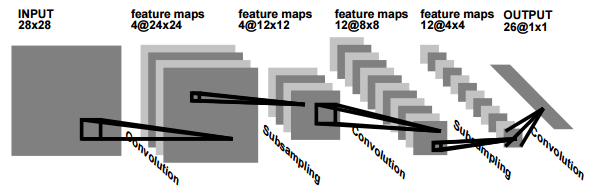
\includegraphics{conv.png}}
\caption{LeNet(the first convolutional neural netowrk) architecture\cite{lecun1995convolutional}}
\label{flr1}
\end{figure}

Convolutional neural network works expertise in extracting features from data with spatial or temporal pattern, usually image or text. 

\chapter{Methodology, procedure, design, etc.}

This may be one chapter or several.  Again, titles should be more
informative than the above.

You will almost certainly need diagrams to clarify your meaning.  The
\LaTeXe\ \texttt{graphics} package allows the inclusion of PostScript
graphics, as in \fig{flr1}.  The inclusion of \LaTeX\ \texttt{picture}
graphics, as in \fig{fzsys}, requires no auxiliary packages and allows
the mathematical formatting features of \LaTeX\ to be used in
diagrams; but the \texttt{picture} files, unlike PostScript files,
usually require manual editing.

\begin{figure}[htbp]
\centerline{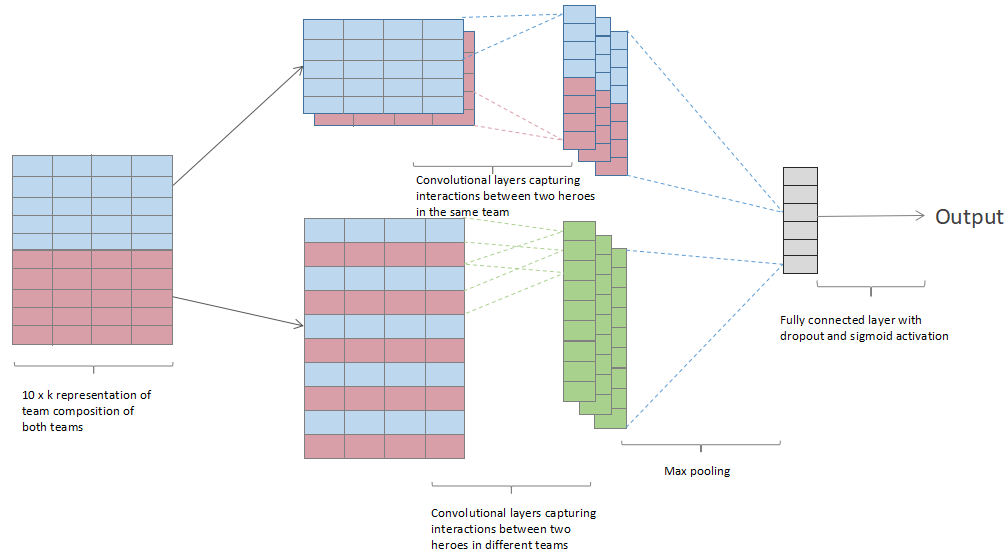
\includegraphics{architecture.png}}
\caption{Experimental two-way active crossover (op-amp version)}
\label{flr1}
\end{figure}

\begin{figure}[htbp]
\caption{Modeling a discrete-time LTI system using $z$-transforms}
\label{fzsys}
\end{figure}

\chapter{Results and discussion \ldots}

\ldots\ or perhaps the discussion should be a separate chapter.

In any case, you will probably need to include tabulated results.
\tab{tf2} illustrates the use of various \LaTeX\ environments to
include a computer printout (plain text file) in a document.  The
\texttt{verbatim} environment, which encloses the formatted text, is
also useful for program listings.

\begin{table}\renewcommand{\baselinestretch}{1.0}
\caption{\sl Fraction of air volume involved in heat exchange for
second mode (right column) vs.\ filling factor (left column).  The
plain-text headings represent $f$, $m$, $\mu_2$ and $f_2$.}
\label{tf2}

\begin{center}
\begin{minipage}[c]{2.85in}\small\normalsize
\begin{verbatim}

 f(%)     m         mu2     f2(%)

 0.016   80.00    0.05400   4.874
 0.031   56.57    0.07732   5.438
 0.062   40.00    0.11103   6.125
 0.125   28.28    0.16001   6.970
 0.250   20.00    0.23175   8.020
 0.500   14.14    0.33799   9.329
 1.000   10.00    0.49789  10.967
 2.000    7.07    0.74444  13.008
 4.000    5.00    1.13919  15.525
 8.000    3.54    1.81095  18.568

19.237    2.28    3.61958  23.174
37.180    1.64    7.28635  27.094
57.392    1.32   14.63631  29.813
74.316    1.16   29.35160  31.453
85.734    1.08   58.79364  32.360
\end{verbatim}
\end{minipage}
\end{center}
\end{table}

\chapter{Conclusions}

\section{Summary and conclusions}

\section{Possible future work}

\appendix

% Chapters after the \appendix command are lettered, not numbered.
% Setting apart the appendices in the table of contents is awkward:

\newpage
\addcontentsline{toc}{part}{Appendices}
\mbox{}
\newpage

% The \mbox{} command between two \newpage commands gives a blank page.
% In the contents, the ``Appendices'' heading is shown as being on this
% blank page, which is the page before the first appendix.  This stops the
% first appendix from be listed ABOVE the word ``Appendices'' in the
% table of contents.

% \include appendix chapters here.

\chapter{Dummy appendix}

Appendices are useful for supplying necessary details or explanations
which do not seem to fit into the main text, perhaps because they are
too long and would distract the reader from the central argument.
Appendices are also used for program listings.

Notice that appendices are ``numbered'' with capital letters, not
numerals.  When the \verb+\appendix+ command in
\LaTeX~\cite[p.\,175]{lamport} is used with the \texttt{book} document
class, it causes subsequent chapters to be treated as appendices.

\chapter{Program listings}

\section{First program}

Some initial explanatory notes may precede the listing.

\section{Second program}

\section{Etc.}

\chapter{Companion disk}

If you wish to make some computer files available to your examiners,
you can list and describe the files here.  The files can be supplied
on a disk and inserted in a pocket fixed to the inside back cover.

The disk will not be needed if you can specify a URL from which the
files can be downloaded.

\cleardoublepage

\newpage
\nocite{*}
\bibliographystyle{ieeetran}
\bibliography{bib}

\end{document}